\chapter{Omisión de palabras}

Anteriormente se especificó que la base de datos de los préstamos serían únicamente palabras de contenido, y a partir de ellas se realizaron los análisis anteriores.  Al trabajar con esta clasificación se están restringiendo a todas las palabras que pueden ser catalogadas como préstamos (algunos artículos o pronombres de un determinado idioma se encuentran en los demás), sin embargo los resultados obtenidos han reflejado contextos históricos en los cuáles explicar el flujo de un idioma a otro, por lo que las restricciones han ayudado a tener deducciones más limpias. 

Por el momento ya no se tratara con la interpretación histórica de las migraciones, se centrará la siguiente parte en suponer a los préstamos como un conjunto donde la propiedad del uso entre idiomas es adecuada, y ver como es afectada la propiedad si se modifica el conjunto. 

La manera de alterar a los prestamos se realizará al hacer restricciones en las palabras que conforman el conjunto, como antecedente se tiene el haber eliminado todas las palabras funcionales  y utilizar las de contenido.  Al tomar como verdaderos a los prestamos acumulados entre idiomas (obtenidos en el capitulo anterior), las restricciones consistirán en eliminar aquellas palabras que comiencen con ciertas letras,  y analizar que ocurre con el uso tras las exclusiones. 

\hfill\break

El proceso es sencillo y consiste en lo siguiente:
 


\begin{enumerate}
	
	\item Se eligen una pareja de idioma origen $\textit{A}$ e idioma receptor $\textit{B}$ y la lista de préstamos acumulados de \textit{A} en \textit{B}.
	
	\item Se escogen de forma aleatoria un conjunto de letras (desde una hasta cuatro), y se eliminan del conjunto de prestamos acumulados  a todas las palabras cuya primer letra sea alguna de las elegidas.  
	
	\newpage
	
	\item Se designan tres conjuntos:
	
		\begin{itemize}
			\item \textbf{Conjunto original:} Conformado por los prestamos acumulados  de $\textit{A}$  en $\textit{B}$.
			\item \textbf{Conjunto reducido:} Conjunto original menos las palabras eliminadas. 
			\item \textbf{Conjunto residuo:} Conformado por las palabras eliminadas del conjunto original. 
		\end{itemize}
	
	\item En cada conjunto se empleo la ecuación \ref{ec.fuso} para obtener el uso de $\textit{A}$ en $\textit{B}$  con los elementos de cada grupo y en todos de búsqueda (1900-2009).
	
	 
	
\end{enumerate}


Por la cantidad de elementos que contiene el conjunto residuo, los valores de uso para este conjunto son pequeños comparados con los obtenidos en el conjunto original o en el reducido, por lo que no se graficaron. Cabe decir que entre mas letras se escojan para reducir el conjunto, el residuo tendrá cada vez más elementos siendo en algún momento comparable al original.  Por ello se decidió que el máximo de restricciones fuese de cuatro letras. 

Se denotan como $V_{i}$ y $v_{i}$ al uso en el año $i$ de los conjuntos original y reducido respectivamente; para saber que tan diferentes son los valores de uso, se calculó el valor promedio $\bar{v}$ de cada $v$  y  se empleó la siguiente ecuación:

\begin{equation}
\label{ec.dif_uso}
R^{2} = 1 - \sum_{i} \frac{ \left( v_{i} - V_{i} \right)^{2}  }{ \left( v_{i} - \bar{v} \right)^{2} }
\end{equation}


Se define el termino \textbf{Conservación del uso} para aquellos pares de idiomas donde el uso de uno en otro no cambie a pesar de las omisiones. Valores de $R^{2}$  próximos a 1 indicarán que el uso se mantiene, y las omisiones no afectaron a los conjuntos, en caso contrario $R^{2}$ tomará valores cercanos a cero.  

Para la presentación de resultados, se graficó en color negro los valores de uso en el conjunto original, sin importar que combinación de idiomas se este tratando.  Para el conjunto reducido, el uso se marcó en color rojo.  En cada grafica se especifica que letras se usaron para las reducciones. 

\newpage

\subsubsection*{Inglés}

\begin{figure}[h!]
	\centering
	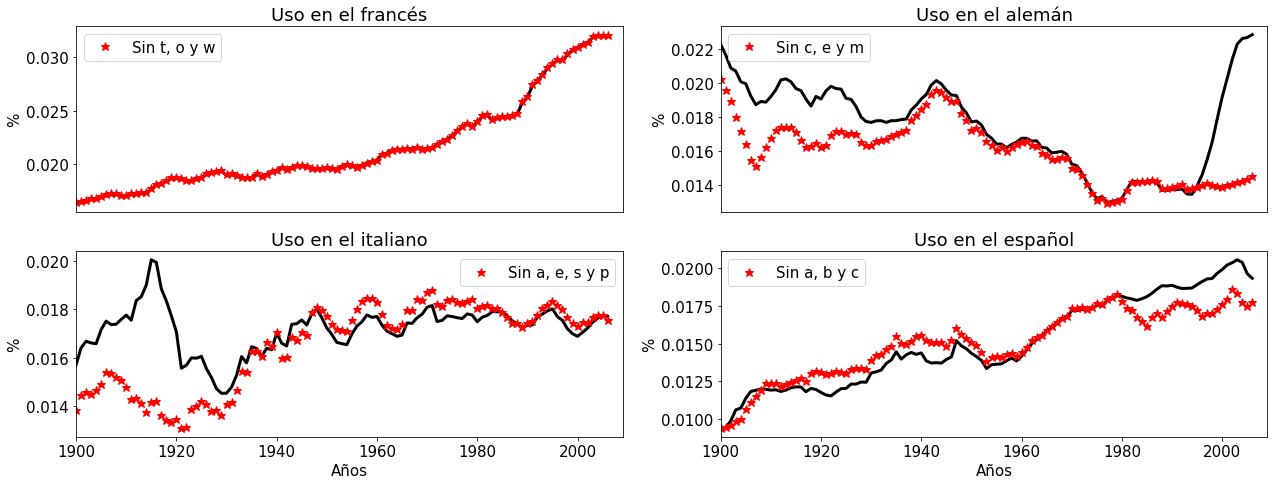
\includegraphics[width=14.5cm, height=6.8cm]{OM_EN.png}
	\label{fig.OM_EN}
	\caption{Omisiones del inglés.}
\end{figure}


\subsubsection*{Francés}

\begin{figure}[h!]
	\centering
	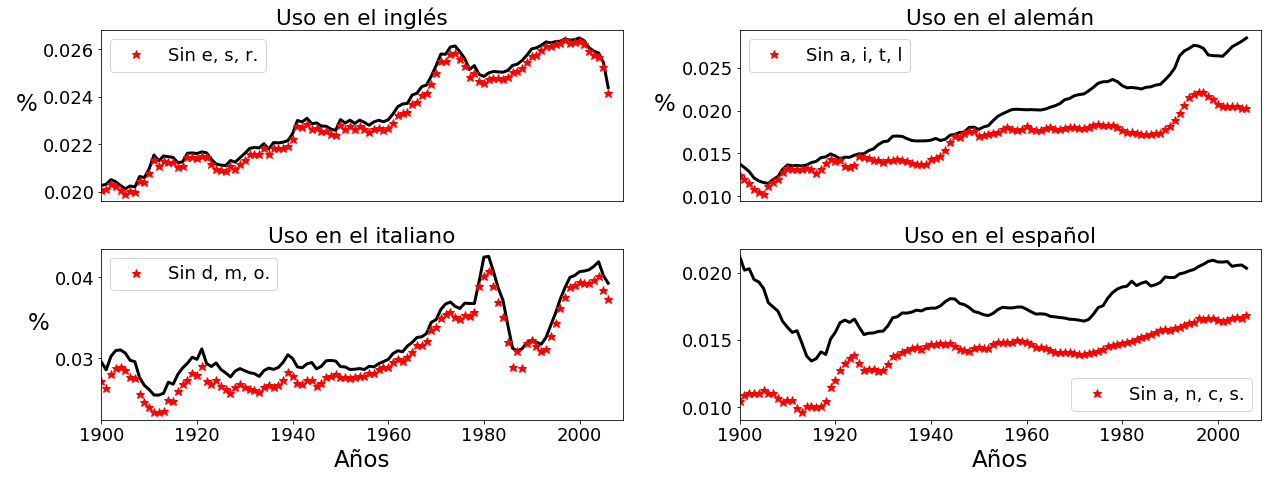
\includegraphics[width=14.5cm, height=6.8cm]{OM_FR.png}
	\label{fig.OM_FR}
	\caption{Omisiones del francés.}
\end{figure}


\newpage
\subsubsection*{Alemán}

\begin{figure}[h!]
	\centering
	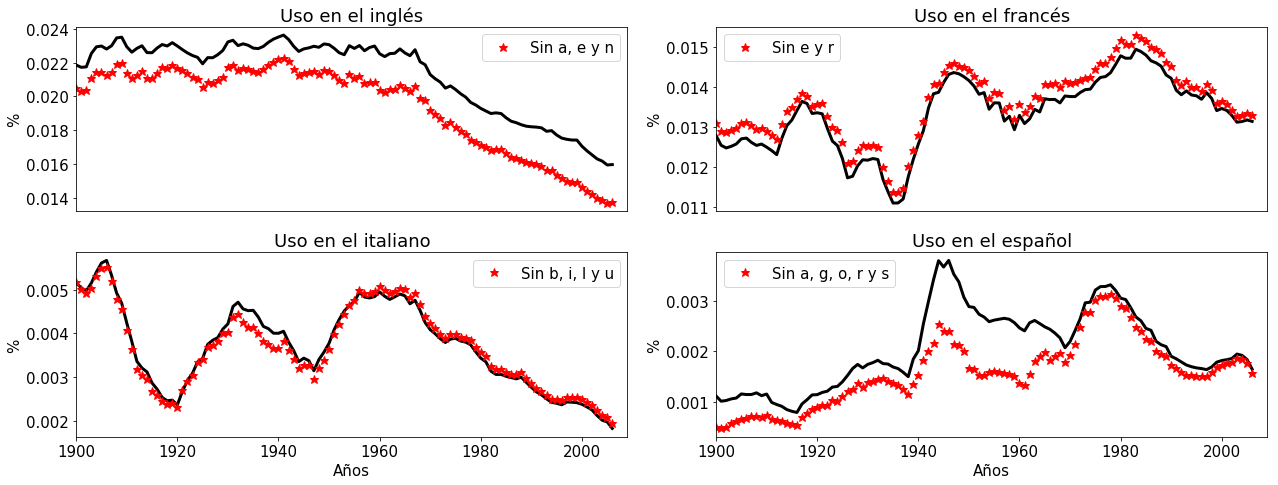
\includegraphics[width=14.5cm, height=6.8cm]{OM_GE.png}
	\label{fig.OM_GE}
	\caption{Omisiones del alemán.}
\end{figure}


\subsubsection*{Italiano}

\begin{figure}[h!]
	\centering
	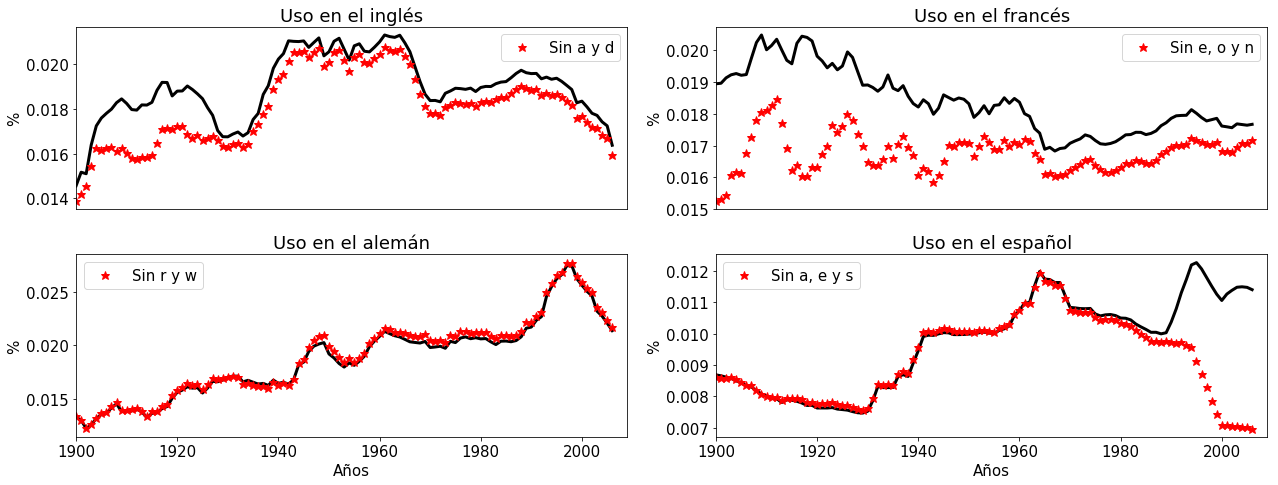
\includegraphics[width=14.5cm, height=6.8cm]{OM_IT.png}
	\label{fig.OM_IT}
	\caption{Omisiones del italiano.}
\end{figure}

\newpage
\subsubsection*{Español}

\begin{figure}[h!]
	\centering
	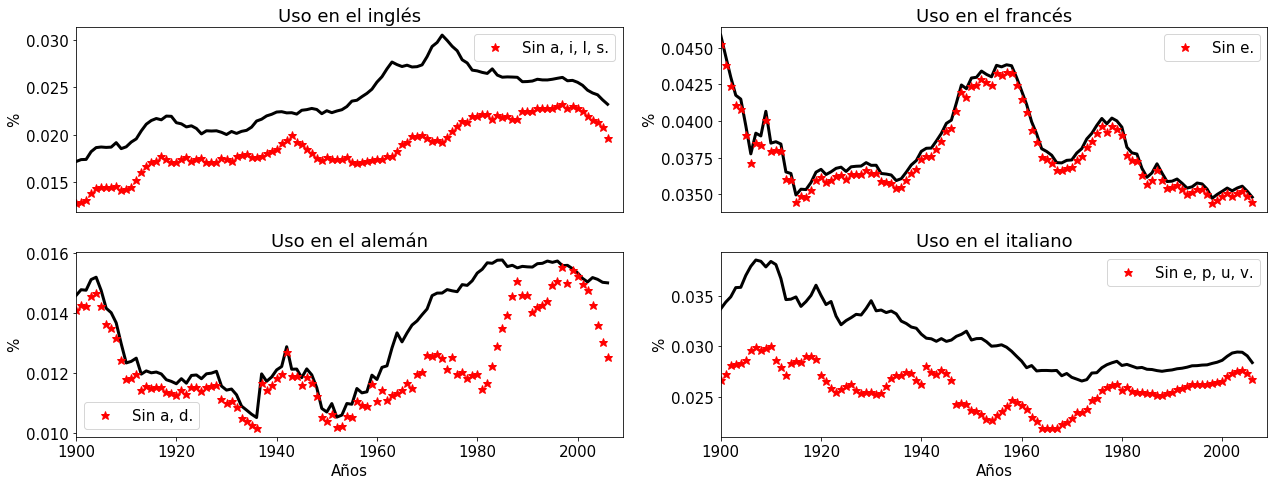
\includegraphics[width=14cm, height=6.8cm]{OM_SP.png}
	\label{fig.OM_SP}
	\caption{Omisiones del español.}
\end{figure}


Tras reducir el corpus de palabras con diferentes condiciones, se distinguieron las siguientes características en el comportamiento de un idioma sobre otro:


\begin{itemize}
	
	\item Valores iguales. Punto a punto el conjunto reducido empalma al original, siendo las gráficas indistinguibles, indicando que el uso se conserva a pesar de las omisiones. 
		
	\item Diferencia de alturas. Ambas gráficas muestran el mismo comportamiento o variaciones en toda la escala de tiempo,  sólo que  en cada año existe una diferencia casi constante entre los valores de una y otra, siendo el uso de las palabras excluidas el valor de diferencia.  En este caso se dirá que el uso también se conserva ya que ambas graficas tienen los mismos valores sólo que están desfasados. 
	
	\item Diferencias por periodos. Una combinación de los puntos anteriores,  donde las graficas son idénticas salvo en algún periodo donde se presenta la diferencia de alturas, indicando la relevancia de los prestamos omitidos en el periodo. 
	
	\item Alteraciones prolongadas. Existen periodos donde el uso del conjunto reducido es completamente diferente al conjunto original. Al igual que en el punto anterior, los préstamos omitidos son los más relevantes en estas etapas ya que sin ellos el uso no se conserva.
			
\end{itemize}


La elección de las letras que se utilizaron para las omisiones y que conllevaron a los resultados fueron completamente aleatorios;  el que una combinación presente alguna de las características mencionadas no significa que sea la misma para otras alternativas en las omisiones. Lo único que se puede confirmar es que sin importar los elementos excluidos, el uso en el conjunto reducido presentará alguna de estas propiedades. 

Para tener resultados íntegros sobre la conservación del uso a partir del valor de $R^{2}$,  se calculó además la diferencia de alturas  promedio $\Delta h$ entre el uso de ambos conjuntos, el cálculo  de $R^{2}$ se realizó al aumentar la altura promedio a cada valor del uso en el conjunto reducido.


\begin{table}[h!]
	\centering
	\begin{tabular}{ccc}
		\textbf{}  & \textbf{$\Delta h$}  & \textbf{$R^{2}$}      \\
		\textbf{inglés-francés}    & 0.001           & 0.99       \\
		\textbf{inglés-alemán}     & 0.003           & 0.91       \\
		\textbf{ingles-italiano}   & 0.004           & 0.63       \\
		\textbf{ingles-español}    & 0.002           & 0.93       \\
		\textbf{francés-inglés}    & 0.001           & 0.98       \\    
		\textbf{francés-alemán}    & 0.003           & 0.84       \\ 
		\textbf{francés-italiano}  & 0.002           & 0.81       \\ 
		\textbf{francés-español}   & 0.003           & 0.81       \\ 
		\textbf{alemán-inglés}     & 0.002           & 0.98       \\
		\textbf{alemán-francés}    & 0.002           & 0.88       \\
		\textbf{alemán-italiano}   & 0.001           & 0.99       \\
		\textbf{alemán-español}    & 0.003           & 0.96       \\
		\textbf{italiano-inglés}   & 0.002           & 0.78       \\
		\textbf{italiano-francés}  & 0.003           & 0.79       \\
		\textbf{italiano-alemán}   & 0.001           & 0.97       \\
		\textbf{italiano-español}  & 0.002           & 0.89       \\
		\textbf{español-inglés}    & 0.004           & 0.85       \\
		\textbf{español-francés}   & 0.001           & 0.99       \\
		\textbf{español-alemán}    & 0.003           & 0.67       \\
		\textbf{español-italiano}  & 0.004           & 0.74       
	\end{tabular}
	\caption{Parámetros de las omisiones.}
	\label{tab.Omision}
\end{table}


A partir de la tabla, se muestra que la mejor similitud entre los conjuntos se da en aquellos donde no hay alteraciones prolongadas; como se menciono anteriormente el que se tenga esta característica entre dos idiomas depende de la elección de palabras que restringen al conjunto, alguna otra combinación modificara las características entre  el conjunto original y el reducido, sin embargo se comprobó con diferentes muestreos que los casos donde hay alteraciones prolongadas son escasos.


\section{Comentarios del método}

El realizar diferentes elecciones para restringir a las palabras que conforman los prestamos de un idioma en otro, mostró desde el punto de vista estadístico que no importan cuales elementos conforman el corpus, la propiedad del uso es la misma, ya que individualmente los valores de uso de una única palabra pueden variar en los años del análisis y ser distintos a los de otra palabra, sin embargo al tratar a todo el conjunto, el uso se comporta de la misma  manera, sin importar los valores individuales de los elementos que lo conforman. 







